\documentclass[runningheads,a4paper]{llncs}

%%% Some recommended packages.
%\usepackage{booktabs}   %% For formal tables:
%                        %% http://ctan.org/pkg/booktabs
%\usepackage{subcaption} %% For complex figures with subfigures/subcaptions
%                        %% http://ctan.org/pkg/subcaption

% Packages usually used by soton
	% Package for input encoding
	\usepackage[utf8]{inputenc}
	
	%\usepackage[T1]{fontenc}
	%\usepackage{lmodern}
	
	% Package for multilingual support, loaded with English support.
	\usepackage[english]{babel}
	
	% Package for fancy quotations
	\usepackage[autostyle]{csquotes}
	
	% Package for URLs
	\usepackage{url}
	
	\usepackage{colourSoton}
	
	% Package for hyper-references
	\usepackage{hyperref}
	\hypersetup{
		colorlinks=true,
		citecolor=red,
		linkcolor=blue,
		urlcolor=cyan,
	}
	
	% Package for graphics
	\usepackage{graphicx}
	\graphicspath{ {img/} }
	
\usepackage[colorinlistoftodos]{todonotes}

% Package for change tracking
	\usepackage{chgtrk}
	\newCTcontributor{Colin}
	\newCTcontributor{Son}
	\newCTcontributor{Karla}
	
 	% Package for abbreviation
 	\usepackage{abbrev-scxml2020}
	
	% Package for standalone source code
	\usepackage{standalone}
	
	% Package for requirements document
%	\usepackage[compact]{reqdoc}
	
	% Package for TikZ pictures
	\usepackage{tikz}
	\usetikzlibrary{positioning}
	\usetikzlibrary{shapes}
	
	% Custom pgf pictures
%	\usepackage{pgf-picture}
	
	\usepackage{wrapfig}
	
	% Package for listing Event-B code
	\usepackage[colour]{lstEventB}

	
% For floating listings
\usepackage{float}
\newfloat{lstfloat}{htbp}{lop}
\floatname{lstfloat}{Listing}
\def\lstfloatautorefname{Listing} % needed for hyperref/auroref
	
	%package for envelope
	\usepackage{bbding}
% end of packages used by soton

\title{Semantics of refinement in SCXML}
\author{Karla Morris \inst{1} 
\and Colin Snook \inst{2} 
\and Thai Son Hoang\inst{2} 
}
\date{August 2020} 

%
% the affiliations are given next; don't give your e-mail address
% unless you accept that it will be published
\institute{
	Sandia National Laboratories, 
	Livermore, California, U.S.A.\\
	% \email{\{knmorri,rob,ghulett\}@sandia.gov}
	\and
	ECS, University of Southampton,
	Southampton, United Kingdom\\
	% \email{\{cfs,t.s.hoang,mjb\}@soton.ac.uk}\\
}

\begin{document}

\maketitle

% !TEX root = ../main.tex
\begin{abstract}
Text of abstract 
\end{abstract}

\section{Introduction}
We formalise the semantics of refinement in SCXML by modelling, in Event-B,
\begin{itemize}
	\item the structure and behaviour of abstract SCXML models,
	\item the structure, behaviour of refined SCXML models and their relationship to abstract models.
	\item We then refine the latter to remove verification artifacts and show that it is no different to the abstract model and hence SCXML refinement can be applied iteratively.
\end{itemize}

Since SCXML consists of a state-chart behaviour superimposed with a 'run to completion' execution semantics, we formalise the refinement of these two parts separately and then compose the two definitions to obtain the complete SCXMl refinement semantics.
% !TEX root = ../main.tex

\section{Background}
\label{sec:background}
 
% !TEX root = ../main.tex

\subsection{Event-B}
\label{sec:eventb}

\EventB~\cite{abrial10:_model_event_b,hoang13:_introd_event_b_model_method} is a formal method for system
design.  It uses \emph{refinement} to introduce system details gradually into the
formal model.  An \EventB model contains two parts: \emph{contexts} and \emph{machines}. 
Contexts contain \emph{carrier sets}, \emph{constants}, and \emph{axioms} constraining 
the carrier sets and constants.  Machines contain \emph{variables} |v|, \emph{invariants} |I(v)| 
constraining the variables, and \emph{events}. An event consists of a guard 
denoting its enabled-condition and an action defining the value of variables after the event is executed.  
In general, an event |e| has the form: |any t where G(t, v) then S(t, v) end| where |t| 
are the event parameters, |G(t, v)| is the guard of the event, and |S(t, v)| is the action of the event.
% \begin{center}
  % |any t where G(t, v) then S(t, v) end|
%& \inlineevent{\Be}{}{\Bt}{G(\Bt,\Bv)}{}{S(\Bt,\Bv)}
% \end{center}
%In the case where the event has no parameters, we use the following form
%\begin{center}
%  |when G(v) then S(v) end|
%%& \inlineevent{\Be}{}{}{G(\Bv)}{}{S(\Bv)}~,
%\end{center}
% and when the event has no parameters and no guard, we use
% \begin{center}
%   |begin S(v) end|
% %& \inlineevent{\Be}{}{}{}{}{S(\Bv)}~.
% \end{center}
%The action of an event comprises of one or more assignments, each of them has one of the following forms: (1) |v := E(t, v)|, (2) |v :: E(t, v)|, and (3) |v :∣ P(t, v)|.  Assignments of form (1) are deterministic, assign the value of expression |E(t, v)| to |v|.  Assignments of forms (2) and (3) are non-deterministic. (2) assigns any value from the set |E(t,v)| to |v|, while (3) assigns any value satisfied predicate |P(t,v)| to |v|.
%A machine in \EventB corresponds to a transition system
%where \emph{variables} represent the states and \emph{events} specify
%the transitions.  Note that invariants |I(v)| are inductive, i.e., they must be \emph{maintained} by all events. This is more strict than general safety properties which hold for all reachable states of the \EventB machine.  
% This is also the difference between verifying the consistency of \EventB machines using theorem proving and model checking (e.g., \PROB) techniques: model checkers explore all reachable states of the system while interpreting the invariants as safety properties.  

Machines can be refined by adding more details.  Refinement can be done by extending the machine 
to include additional variables (\emph{superposition refinement}) representing new features of 
the system, or by replacing some (abstract) variables by new (concrete) variables (\emph{data refinement}).  
% More information about \EventB can be found
% in~\cite{hoang13:_introd_event_b_model_method}.
Refinement in \EventB is reasoned on an event basis.  
A (concrete) event |f| refines an (abstract) event |e| if whenever |f| is enabled then |e| is also enabled (guard strengthening), and the action of |f| is the same or equivalent to |e| (where equivalence is given by some relationship defined in the invariants). 
New events are said to refine `skip' (an implicit abstract event that did nothing), and therefore do not alter abstract variables.
 More information about \EventB refinement can be
found in~\cite{abrial10:_model_event_b}.
\EventB is supported by the Rodin Platform (Rodin\footnote{An extensible toolkit which includes 
facilities for modelling, verifying the consistency of models using theorem proving and model 
checking techniques, and validating models with simulation-based approaches.})~\cite{abrial10:_rodin}.

\hl{Proof obligations are generated to ensure the consistency of
  \mbox{\EventB} models.  An important proof obligation in
  \mbox{\EventB} is invariant preservation to prove that safety
  properties (encoded as invariants of the models) will not be
  violated for any reachable states.  In this paper, we also make use
  of other proof obligations in \mbox{\EventB} such as (relative)
  deadlock-freeness and (conditional) event convergence to construct
  our proof of liveness properties under some fairness
  assumptions.%
}

\hl{%
  For the trace semantics corresponding to \mbox{\EventB} machines and
  the interpretation of LTL properties over traces, we refer the readers
  to \mbox{\cite{hoang2016ltl}}.  Here, we recall the notation for
  fairness assumptions underlying event-based formalisms such as
  \mbox{\EventB~\cite{lamport1977proving,hudon16:_unit_b_method}}. Given
  an event \mbox{\EventBInline{e}}, a weak-fairness assumption
  \mbox{\EventBInline{WF(e)}} states that if \mbox{\EventBInline{e}}
  is enabled continually, then it must occur infinitely often.
  Similarly, a strong-fairness assumption \mbox{\EventBInline{SF(e)}}
  states that if \mbox{\EventBInline{e}} is enabled infinitely often,
  then it must occur infinitely often. Formally,
}
\begin{center}
  \EventBInline{WF(a)  <=> (FG enabled(e) => GF [e])}, and

  \EventBInline{SF(a)  <=> (GF enabled(e) => GF [e])},
\end{center}
\hl{%
  where \mbox{\EventBInline{G}} and \mbox{\EventBInline{F}} are the
  temporal operators denoting \emph{globally}, and \emph{finally},
  respectively; and \mbox{\EventBInline{enabled(e)}} denotes that
  event \mbox{\EventBInline{e}} is enabled and
  \mbox{\EventBInline{[e]}} denotes an occurrence of event
  \mbox{\EventBInline{e}}.
}
% In \EventB the run to completion pseudocode of Listing~\ref{lst:scxml-r2c} could be represented (somewhat abstractly) as shown in Listing~\ref{lst:eventb-r2c}.
% \begin{lstlisting}[caption={Run to completion pseudocode in \EventB},label={lst:eventb-r2c}, language=Event-B, escapechar=|, frame=single, float=t]
%  FireUntriggered // Fire  enabled un-triggered transitions
% when
%     UC = FALSE // Has not yet completed firing un-triggered transitions
%     untriggered() /= {}
% then
%     execute(untriggered()) // Execute enabled un-triggered transitions
% end
% UntriggeredCompleted // Un-triggered transitions are completed
% when
%     UC = FALSE // Has not yet completed firing un-triggered transitions
%     untriggered() = {} // No more enabled un-triggered transitions
% then
%     UC = TRUE // Complete firing un-triggered transitions
% end
% FireInternallyTriggered // Fire an internal trigger
% when
%     UC = TRUE // Complete firing un-triggered transitions
%     IQ /= {} // The internal triggers queue is non-empty
% then
%     execute(IQ.dequeue) // Execute and dequeue from the internal triggers queue
%     UC := FALSE // Re-enable firing of un-triggered transitions
% end
% FireExternallyTriggered // Fire an external trigger
% when
%     UC = TRUE // Complete firing un-triggered transitions
%     IQ = {} // The internal trigger queue is empty
%     EQ /= {} // The external trigger queue is non-empty
% then
%     execute(EQ.dequeue)  // Execute and dequeue from the external triggers queue
%     UC := FALSE // Re-enable firing of un-triggered transitions
% end
% \end{lstlisting}	
% Here, |IQ| and |EQ| are queues of internally and externally, raised triggers, |untriggered| selects a set of currently enabled un-triggered transitions, |dequeue| retrieves the next trigger from the given queue and selects the set of transitions that become enabled by it and |execute| fires the given set of transitions. 
% Note that this is an abstract representation where each event (|FireUntriggered|, |FireInternallyTriggered|, and |FireExternallyTriggered|) would be specialised to select a particular set of transitions that can be fired in parallel and |execute()| would be replaced by actions that encode the state changes made by those transitions.
% Representing the condition \textbf{untriggered\_enabled} (Line 3 in Listing~\ref{lst:scxml-r2c}) is cumbersome since we would need to write a conjunction of all the possible un-triggered guards. Instead we introduce a dummy un-triggered event that is only fired when no other selection of un-triggered transitions are available and sets a boolean flag, |UC|, to indicate that none of the real un-triggered events was fired and a trigger needs to be consumed.
 
% Note that causing all of the
% transitions to simultaneously and atomically fire for each event is a
% further semantic choice.  Transitions associated with |FireUntriggered|,
% |FireInternallyTriggered|, and |FireExternallyTriggered| might
% just as well fire separately in a non-deterministic order, or by use
% of a per-transition priority, fire in a predetermined order.  Each
% choice has realistic exemplars in the physical world, and to some
% degree, the choice is arbitrary.  The argument in favour of the
% parallel atomic transitions chosen here is pragmatic: the resulting
% representation in \EventB is more terse.

%%% Local Variables:
%%% mode: latex
%%% TeX-master: "../main"
%%% End:

% !TEX root = ../main.tex

\subsection{UML-B State-machines}
\label{sec:iumlb}

\UMLB~\cite{said15:umlbSosym,snook14:iumlbStatem,snook06umlbTosem} provides a diagrammatic modelling notation for \EventB in the form of state-machines and class diagrams. 
The diagrammatic models relate to an \EventB machine and generate or contribute to parts of it. 
For example a state-machine will automatically generate the \EventB data elements (sets, constants, axioms, variables, and invariants) to implement the states. 
Transitions contribute further guards and actions representing their state change, to the events that they elaborate.  
State-machines are typically refined by adding nested state-machines to states.
% Figure~\ref{fig:iumlb-sm} shows an example of a simple state-machine with two states.
% \begin{figure}[!h]
% 	\vspace{-.5cm}
% 	\centering
% 	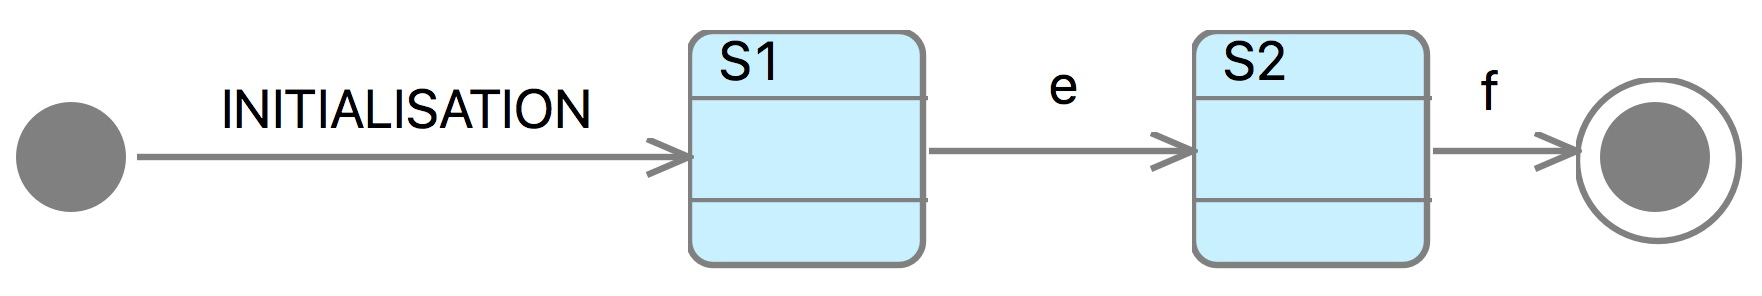
\includegraphics[width=0.6\textwidth]{figures/iumlb-SM}
% 	\caption{An example \UMLB state-machine}
% 	\label{fig:iumlb-sm}
% 	\vspace{-.5cm}
% \end{figure}

Each state is encoded as a boolean variable and the current state is indicated by one of the boolean variables being set to |TRUE|. 
An invariant ensures that only one state is set to |TRUE| at a time.
%The state-machine, is initialised by setting one state variable to |TRUE| and all others to |FALSE|.
Events change the values of state variables to move the |TRUE| value according to the transitions in the state-machine.  
% The \EventB translation%
% %
% \footnote{%
%   Here, $\mathrm{partition(S, T1, T2, \ldots)}$ means the set $S$ is partitioned into disjoint (sub-)sets $T1, T2, \ldots$.
% that cover $S$} 
% of the state-machine in Figure~\ref{fig:iumlb-sm} can be seen in Listing~\ref{lst:eventb-sm}.
% \UMLB also provides the option of an alternative translation with a single state variable ranging over an enumerated type of states, however, the boolean representation of each state is more natural for a user to reference in \SCXML guards and actions.
	
While the \UMLB translation deals with the basic data formalisation of state-machines it differs 
significantly from the semantics discussed in this manuscript. 
\UMLB adopts \EventB's simple guarded action semantics and does not have a concept of triggers and run-to-completion.
Here we make use of \UMLB's state-machine translation but provide a completely different semantic by generating a behaviour into the underlying \EventB events that are linked to the generated \UMLB transitions.
% \begin{lstlisting}[caption={Translation of the state-machine in Fig.~\ref{fig:iumlb-sm}},label={lst:eventb-sm}, language=Event-B, escapechar=|, frame=single]
% variables S1 S2
% invariants 
% 	TRUE !: {S1, S2} => partition({TRUE}, {S1}/\{TRUE}, {S2}/\{TRUE})
% events
%     INITIALISATION: begin S1, S2 := TRUE, FALSE end
%     e: when S1 = TRUE then S1, S2 ≔ FALSE, TRUE  end
%     f: when S2 = TRUE then S2 := FALSE end
% end
% \end{lstlisting}
%%% Local Variables:
%%% mode: latex
%%% TeX-master: "../main"
%%% End:

% !TEX root = ../main.tex

\subsection{SCXML}
\label{sec:scxml}

\SCXML is a modelling language based on Harel statecharts with facilities for adding data elements that are manipulated by transition actions and used in conditions for their firing. \SCXML follows the usual `run to completion' semantics of such statechart languages, where trigger events\footnote{In \SCXML the triggers are called `events', however, we refer to them as `triggers' to avoid confusion with \EventB} may be needed to enable transitions. Trigger events are queued when they are raised, and then one is de-queued and consumed by firing all the transitions that it enables, followed by any (un-triggered) transitions that then become enabled due to the change of state caused by the initial transition firing. This is repeated until no transitions are enabled, and then the next trigger is de-queued and consumed. There are two kinds of triggers: internal triggers are raised by transitions and external triggers are raised by the environment (spontaneously as far as our model is concerned). An external trigger may only be consumed when the internal trigger queue has been emptied. 

\begin{lstlisting}[caption=Pseudocode for 'run to completion',label={lst:scxml-r2c}, frame=single]
while running:
	while completion = false
		if untriggered_enabled
			execute(untriggered())
		elseif IQ /= {}
			execute(internal(IQ.dequeue)) 
		else
			completion = true
		endif
	endwhile
	if EQ /= {}
		execute(EQ.dequeue) 
		completion = false
	endif
endwhile 
\end{lstlisting}

Listing~\ref{lst:scxml-r2c} shows a pseudocode representation of the run to completion semantics as defined within the latest W3C recommendation document~\cite{scxmlwebsite}. Here IQ and EQ are the triggers present in the internal and external queues respectively. We adopt the commonly used terminology where a single transition is called a \emph{micro-step} and a complete run (between de-queueing external triggers) is referred to as a \emph{macro-step}.

%%% Local Variables: 
%%% mode: latex
%%% TeX-master: "../main.tex"
%%% End: 


%%% Local Variables:
%%% mode: latex
%%% TeX-master: "../main"
%%% End:

\section{Refinement in SCXML}

What can we do in a refinement
\begin{itemize}
	\item add nested state-machine
	\item strengthen guard of transition to new sub-state
	\item strengthen action of transition to new sub-state
	\item add new external trigger
	\item add new internal trigger (can be raised non-determinstically or by a transition
	\item add new triggered or untriggered transition
	\item 
\end{itemize}

what we can not do
\begin{itemize}
	\item cannot change the triggering of a refined transition - i.e. if it is untriggered it always will remain untriggered and if triggered, that trigger will never be changed.
	\item refined transitions cannot raise more internal triggers except newly introduced ones. I.e. when the trigger is first introduced, transitions that do not raise it, never will. (has to do with finalisation)
\end{itemize}

\section{The semantics of refining State-machines in general}

\ColinInlineComment{Describe the  State-machine semantics model - note that we simplified.. we did not deal with parallel regions}

\section{The semantics of refining an SCXML Run to Completion}

To define the SCXML run to completion execution we first define the static elements involved: 
Triggers are partitioned into either Internal or External triggers
|partition (TRIGGERS, InternalTriggers, ExternalTriggers, {nullTrigger})|
A null trigger |nullTrigger| is introduced for convenience to simplify the definition of the initial condition: the execution begins by firing untriggered transitions which is otherwise only done after a trigger is consumed. Hence the null Trigger is said to be consumed during initialisation.

We define the internal and external trigger queues as subsets of internal, resp. external triggers
|	InternalQueue = ℙ(InternalTriggers)|
|	ExternalQueue = ℙ(ExternalTriggers)|

\ColinInlineComment{THIS NEEDS COMPLETING}


\section{The semantics of refining SCXML models}
\ColinInlineComment{This is some old text.. needs updating for our latest approach}

To model the complete \SCXML refinement semantics we now combine the previous two models. 
That is, using the inclusion mechanism built into CamilleX, we combine our models of scxml execution with our models for state-machines.

\subsection{M1 - refinement of combined scxml and state-machine }
For this stage we include the corresponding M1 stages for SCXML and state-machine.

The gluing context defines the needed refinement relationship between concrete and abstract parts of the model.
\begin{enumerate}
	\item \label{item:triggeredness} For transitions that refine abstract transitions, the transition is triggered if and only if its corresponding abstract transition is triggered.
	\item For \emph{triggered} transitions that refine abstract transitions, the trigger is the same as that of the corresponding abstract transition.
	\item For \emph{finalised} transitions that refine abstract \emph{finalised} transitions, the transition source is the same as that of the corresponding abstract transition. I.e. you cannot strengthen the source of an already finalised transition.
	\item the abstract \emph{finalised} transitions are a subset of the abstract transitions that correspond to concrete finalised transitions. I.e. once transitions are finalised they stay finalised in refinements. 
\end{enumerate}
Initially, for item \ref{item:triggeredness} we defined a single axiom giving the equality of the domains of the abstract and concrete transition-trigger relationship.
However, this was insufficient to prove the guard strengthening of the untriggered refined transitions because the |transition_link| relationship is not injective.
(I.e. in general, an abstract transition could be refined by more than one concrete transition)
Instead, we defined two axioms, universally quantifying over the set of refined transitions that are/are not triggered, with the consequent that the corresponding abstract transitions are/are not triggered.
These axioms were sufficient to automatically discharge the guard strengthening POs for both triggered and untriggered refined transitions.

\subsection{M2 - merging old and new events}
We found a problem when we tried to merge the refined and new  transitions of the combined scxml and statechart semantics. 
The problem occurs for merging both triggered and untriggered transitions.
The problem is that we have not considered the case of merging a new state-machine transition with an old refined scxml triggered transition.
Probably this is nonsensical and we should add guards to prevent it.
Ok for triggered but for untriggered our way of distinguishing refined scxml untriggered transitions is via the disappearing variable dqaux

\section{Conclusion}

In conclusion ...

\vspace{6 pt}
\begin{scriptsize}
	
	\par
	\noindent
	All data supporting this study are openly available from the University of Southampton repository at
	https://doi.org/....tbd\\
	
	\par
	\noindent
	\textbf{Acknowledgements} Sandia National Laboratories is a multimission laboratory managed and operated by National Technology \& Engineering Solutions of Sandia, LLC, a wholly owned subsidiary of Honeywell International Inc., for the U.S. Department of Energy’s National Nuclear Security Administration under contract DE-NA0003525.
	
\end{scriptsize}


\bibliographystyle{splncs04}
\bibliography{SCXMLREF}

\end{document}

%%% Local Variables: 
%%% mode: latex
%%% TeX-master: t
%%% End: 
